\documentclass{article} 

\usepackage{amsmath}
\usepackage{mathtools}
\usepackage{amssymb}
\usepackage{xfrac}
\usepackage[margin=1.00in]{geometry}
\usepackage{tabto}
\usepackage{tikz}
\usepackage{pgfplots}


\pgfplotsset{compat = newest}

\title{Testing for plots and whatnot}
\author{Lucas Johnston and Brendan }
\date{\today}

\begin{document}

    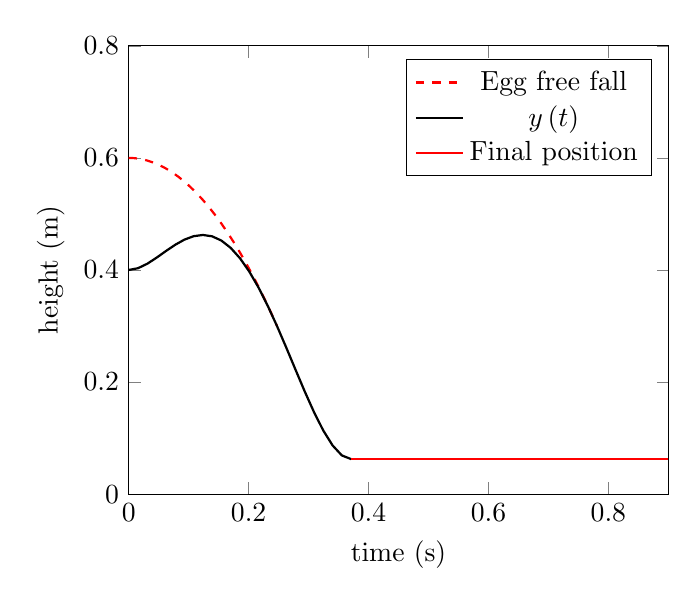
\begin{tikzpicture}
        \begin{axis}[
                xmin = 0,
                xmax = 0.9,
                ymin = 0,
                ymax = 0.8,
                xlabel = time (s),
                ylabel = height (m),
                legend pos=north east, 
                ]
            \addplot[domain = 0:0.247298674822, thick, dashed, red]{0.6-0.5*9.81*x^2};
            \addplot[domain = 0:0.37095212, thick]{160.3981*x^4-105.7772*x^3+14.7141*x^2+0.4};
            \addplot[domain = 0.37095212:0.9, red, thick]{0.0625198478831};
            \legend{Egg free fall, $y\left(t\right)$, Final position};
        \end{axis}
    \end{tikzpicture}   
\end{document}
